% a line starting with "%" is a comment;
%that is, everything following "%" onthe saem line has no impact on the generated .pdf

%document on A4 sized paper with fontsize 12
\documentclass[12pt,a4paper]{article}

%font encoding (no need to pay attention to this)
\usepackage[T1]{fontenc}
\usepackage[utf8]{inputenc}

%packages for mathematical symbols and environments
\usepackage{amsmath,amssymb,amsthm}

%decent margins
\usepackage{geometry}
\geometry{tmargin=2.5cm,bmargin=2.5cm,lmargin=2.5cm,rmargin=2.5cm}

%decent line spacing
\usepackage{setspace}
\onehalfspacing

% package that allows including grapics
\usepackage{graphicx}

%package for formatting urls 
\usepackage{url}

%bibliography is done with natbib and uses the "Author (year)" style
\usepackage[authoryear]{natbib}

%avoids a faint print problem on some systems
\usepackage{ae,aecompl}

%define some mathematical environments
\newtheorem{lemma}{Lemma}
\newtheorem{proposition}{Proposition}
\newtheorem{example}{Example}
\newtheorem{assumption}{Assumption}
\newtheorem{result}{Result}
\newtheorem{theorem}{Theorem}
\newtheorem{corollary}{Corollary}
\newtheorem{definition}{Definition}

%%%%%%%%%%%%%Nice formatting of (sub)section headings (no need to pay attention)
\makeatletter
\renewcommand{\section}{\@startsection{section}{1}{0mm}{-1.5\baselineskip}{0.8\baselineskip}{\normalfont\large\centering}}
\renewcommand{\subsection}{\@startsection{subsection}{2}{0mm}{-0.1\baselineskip}{0.5\baselineskip}{\normalfont\bf\flushleft}}
\renewcommand{\section}{\@startsection{section}{1}{0mm}{-0.9\baselineskip}{0.5\baselineskip}{\normalfont\large\centering}}
\renewcommand{\subsection}{\@startsection{subsection}{2}{0mm}{-0.1\baselineskip}{0.3\baselineskip}{\normalfont\bf\flushleft}}
\renewcommand{\@seccntformat}[1]{\csname the#1\endcsname
\hspace{+0mm}\large{.}\hspace{+1.9mm}}
\renewcommand{\@seccntformat}[2]{\csname the#1\endcsname
\hspace{+0mm}\large{.}\hspace{+1.9mm}}
\makeatother
%%%%%%%%%%%%

%%%%%%%%%%%%%%%%%%%%%%%%%%%%%%%%%%%%%%%%%%%%%%%
%%%%%%%%%%%%%% Frontmatter %%%%%%%%%%%%%%%%%%%%
%%%%%%%%%%%%%%%%%%%%%%%%%%%%%%%%%%%%%%%%%%%%%%% 

% You  have to fill in the right information below

\title{Your Title}
\author{Your Name}
\date{\today} %you can use something like \date{August 17, 2017} to get a date that is not today's date


%%%%%%%%%%%%%%%%%%%%%%%%%%%%%%%%%%%%%%%%%%%%%%
%%%%%%%%%%%%% DOCUMENT %%%%%%%%%%%%%%%%%%%%%%%
%%%%%%%%%%%%%%%%%%%%%%%%%%%%%%%%%%%%%%%%%%%%%%

\begin{document}

%"\maketitle" inserts title, author and date into the document
\maketitle

\section{Introduction}\label{sec:intro}

Here goes your introduction. This document can be used as a template (in this case you want to delete all my text from here to the \verb|\bibliographystyle{chicago}| comand) but I will also give some examples of how to cite and reference, and how to use mathematics in \LaTeX. Ideally, you should look at the .pdf and the .tex file at the same time to see what the code generates. 

\subsection{Literature Review}\label{sec:literature}

The literature review goes here. Let me give some examples how to cite in \LaTeX\ using BibTeX: The ``Chicago view'' of privacy is based on \cite{stigler1980introduction} and \cite{posner1981economics}. A page in a book  is cited as \citet[p. 34]{solove2010privacy}. Note that all the cited articles, books etc. have to have an entry in the .bib file where you define the label used for citing and store all the information necessary for creating the reference list at the end of the document. You can usually copy and paste the entries for the .bib file from Google Scholar or JSTOR (and otherwise you do it by hand following Martin Osborne's guide).

The advantage of BibTeX is twofold: First, you spell the author names and the publication years correctly. Second, the reference list is automatically generated and formatted nicely.

\section{Model}\label{sec:model}

Mathematics within a line of text is put between \$ marks. For example, \verb|$\frac{3}{4}$| yields the fraction $\frac{3}{4}$ or $\lim_{x\rightarrow \infty}e^{-x}=0$ is generated by\\ % "\\" forces a linebreak; you should normally not use it
\verb|$\lim_{x\rightarrow \infty}e^{-x}=0$|. Subindeces as in $x_1$ are written as \verb|$x_1$|. Here is how you use math environments:

\begin{definition}[Fixed Point]\label{def:fp}
  Let $f: \,D\rightarrow R$ where $D\subseteq R$. If $f(x)=x$, then $x$ is called a \emph{fixed point} of $f$.
\end{definition}

You reference the definition as ``definition \ref{def:fp}'' (that is \verb|definition \ref{def:fp}| in the source file where \verb|def:fp| is the label of the definition above). Similarly, you can reference sections as \verb|section \ref{sec:intro}| which yields ``section \ref{sec:intro}''. Also subsection \ref{sec:literature} can be referenced using \verb|subsection \ref{sec:literature}|. The advantage of such references over writing ``section 1.1'' directly is that your references will automatically adjust if you change something in the structure of your document; for example, if you insert another section.
(Note that you have to compile \LaTeX\ twice before it gets a new reference properly formatted.)

\section{Results}\label{sec:results}


A mathematical result, like a proposition, is written in a similar environment as a definition.

\begin{proposition}\label{prop:fp01}
  Let $f: \,[0,1]\rightarrow[0,1]$ be an increasing function. Then, $f$ has a fixed point.
\end{proposition}

\section{Your Extension}\label{sec:ext}

You can include a graphic with the command \verb|\includegraphics{filename}| (recommended file formats are png, eps or pdf). Usually it is a good idea to place the graphic in a figure environment as here:

\begin{figure}[h]
  \centering
  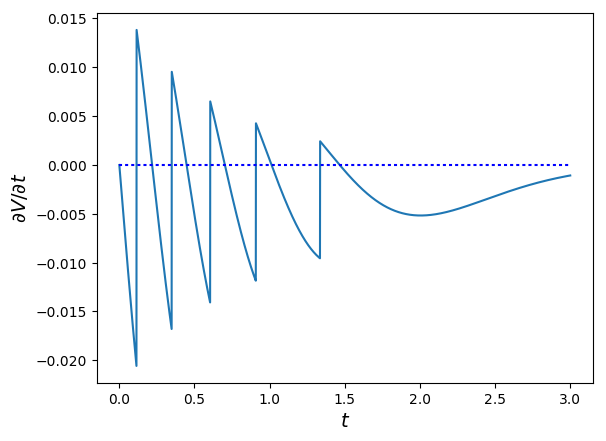
\includegraphics[scale=0.6]{Vprime}
  \caption{A nice figure}
  \label{fig:zigzag}
\end{figure}

We can reference the figure as figure \ref{fig:zigzag} using its label.

Sometimes you need to have a nicely formatted table. See \url{https://en.wikibooks.org/wiki/LaTeX/Tables} for this.

\section{Conclusion}

All scientific writing should be done in \LaTeX.

\newpage

%\section*{name} creates a section without section number
\section*{Appendix}
\noindent\textbf{Proof of proposition \ref{prop:fp01}:} Let 
\begin{equation} \label{eq:A}
A=\{x:\;x\geq f(x)\}.
\end{equation}
Note that $0\in A$ and therefore $A\neq\emptyset$. Let $x^*=\sup A$. Then $f(x^*)\geq x^*$ by the definition of $A$, see equation (\ref{eq:A}), and because $f$ is increasing.

Also $f(x^*)\leq x^*$: if not, i.e. $f(x^*)>x^*$, then $x^*+\varepsilon  > f(x^*+\varepsilon )$ for some $\varepsilon \in(x^*,f(x^*) ]\cap [0,1]$ because $f$ is increasing which contradicts the definition of $x^*$. Hence, $x^*=f(x^*)$.\qed

\newpage

%style of the bibliography
\bibliographystyle{chicago}
%name of the .bib file that has to be in the same folder as this .tex file
\bibliography{privacy}


\end{document}